%% lensing.tex

In the early days of modern science, Newton suspected light could be deflected
by massive bodies, which would imply light consists of particles
\sidecite{Newton1704}.  His contemporary Huygens however convincingly
demonstrated the conformity of light within a coherent wave theory, thereby
explaining phenomena such as reflection, refraction, and polarisation of light
\sidecite{Huygens1690}.  Nowadays, we know both concepts may be used as
descriptions for light.  Similarly, the phenomenon of gravitational lensing can
be thought of as either the delaying and folding of wavefronts, or the curving
of light-particle geodesics.  While both concepts are equivalent, the
multiplicative imaging of light sources seems more intuitive in the wavefront
picture.

Thus, let us consider an arbitrary path of a light ray along a wavefront through
a gravitational potential $\Phi$ with travel time
%
\begin{equation}\eqlbl{travel_time}%
  t = \int \frac{\mathrm{d}\lambda}{v}
\end{equation}%
%
where $\lambda$ is the parametrisation along the path, and $v$ is its speed
which is slower than the speed of light in unperturbed spacetime $(c=1)$ due to
the delay caused by the gravitational potential.  
The Poisson equation connects the gravitational potential to a mass-density distribution
%
% \begin{equation}\eqlbl{Poisson}%
%   \Delta\Phi = 4\pi G\rho.
% \end{equation}%
%
\begin{equation}\eqlbl{Poisson}%
  \Delta\Phi = 4\pi\rho.
\end{equation}%
%
which is commonly called the 'lens'.  Fermat's principle\sidenote{which ---as it
turns out--- can be directly translated from Newtonian physics to general
relativity as shown by e.g.  \citeay{Nityananda1992}.} tells us that the travel
time for such a light ray passing through the lens is stationary with respect to
small variations in its path.  In addition, these paths have to move along null
geodesics on any stationary or non-stationary metric.  In an astrophysical
setting, gravitational potentials are usually non-relativistic\sidenote{the
Sun's potential for example is at its edge around $\Phi \sim 2\times10^{-6}$.},
i.e. $\Phi \ll 1$, and only weakly perturb the flat, unperturbed Minkowski
metric $h_{\mu\nu} = ({1}\,{-1}\,{-1}\,{-1})\cdot\mathbb{1}$.  Thus, we can
write the metric and its line element as
%
% \begin{equation}%
%   \begin{aligned}%
%     g_{\mu\nu} &= h_{\mu\nu} + \frac{2\Phi}{c^{2}}\delta_{\mu\nu} \\
%     \mathrm{d}s^{2} &= g_{\mu\nu}\mathrm{d}x^{\mu}\mathrm{d}x^{\nu}
%      = \left(1+\frac{2\Phi}{c^{2}}\right) c^{2}\mathrm{d}t^{2}
%      - \left(1-\frac{2\Phi}{c^{2}}\right) \mathrm{d}\bm x^{2}.
%   \end{aligned}%
% \end{equation}%
%
\begin{equation}\eqlbl{metric}%
  \begin{aligned}%
    g_{\mu\nu} &= h_{\mu\nu} + 2\Phi\delta_{\mu\nu} \\
    \mathrm{d}s^{2} &= g_{\mu\nu}\mathrm{d}x^{\mu}\mathrm{d}x^{\nu}
     = \left(1+2\Phi\right) \mathrm{d}t^{2} 
     - \left(1-2\Phi\right) \mathrm{d}\bm x^{2}.
  \end{aligned}%
\end{equation}%
%
where $\delta_{\mu\nu}$ is the Kronecker symbol and describes the trace of the
metric.  Since light propagates on null geodesics with $\mathrm{d}s = 0$, we get
%
% \begin{equation}%
%   \frac{1}{v} = \frac{c\mathrm{d}t}{\mathrm{d}\bm x} 
%   = \frac{\sqrt{1 - \frac{2\Phi}{c^{2}}}}{\sqrt{1 + \frac{2\Phi}{c^{2}}}}
% \end{equation}%
%
\begin{equation}\eqlbl{refraction_index}%
  \frac{1}{v} = \left|\frac{\mathrm{d}\bm x}{\mathrm{d}t}\right|^{-1}
  = \sqrt{\frac{1 - 2\Phi}{1 + 2\Phi}} \approx 1 - 2\Phi.
\end{equation}%
%
Moreover, the direction of the light path changes at a rate proportional to the
gradient perpendicular to $\bm v$, which means the total deflection is the
integrated change along the path  
%
% \begin{equation}%
%   \bm\alpha = - \int \left(v \nabla\frac{1}{v}\right)\mathrm{d}\lambda 
%    \approx \frac{2}{c^{2}} \int\nabla\Phi\,\mathrm{d}\lambda
% \end{equation}%
%
\begin{equation}\eqlbl{deflections}%
  \bm\alpha = - \int \left(v \nabla\frac{1}{v}\right)\mathrm{d}\lambda 
   \approx 2 \int\nabla\Phi\,\mathrm{d}\lambda
\end{equation}%
%
The travel-time difference along the perturbed path due to the locally slower
speed of light in comparison to its speed in non-dilated spacetime is called the
\textit{Shapiro delay} \sidecite{Shapiro1964}
%
% \begin{equation}%
%   \Delta t_{\text{Shapiro}} = \int\left(\frac{1}{v}-\frac{1}{c}\right)\mathrm{d}\lambda
%    = -\frac{2}{c^{3}}\int\Phi\,\mathrm{d}\lambda.
% \end{equation}%
%
\begin{equation}\eqlbl{shapiro}%
  \Delta t_{\text{Shapiro}} = \int \left(\frac{1}{v}-1\right)\mathrm{d}\lambda
   = -2\int\Phi\,\mathrm{d}\lambda.
\end{equation}%
%
In general relativity, delays and deflections --- notions of space and time ---
are dependent on the reference frame used.  Since observations of gravitational
lensing are by nature in the observer frame, it makes sense to derive lensing
properties in that frame.  To that end, we now consider the travel times of all
paths from the source to the observer's entire sky\sidenote{The observer sees a
2D surface!}.  The observer at the end of these light paths can only detect
lensed images at certain angular positions $\bm\theta$ on the sky, which are at
a normal direction to the wavefronts (a direct consequence of Fermat's
principle), originating from a source at an unobservable angle $\bm\beta$.

\begin{figure}[h]%
  \centering%
  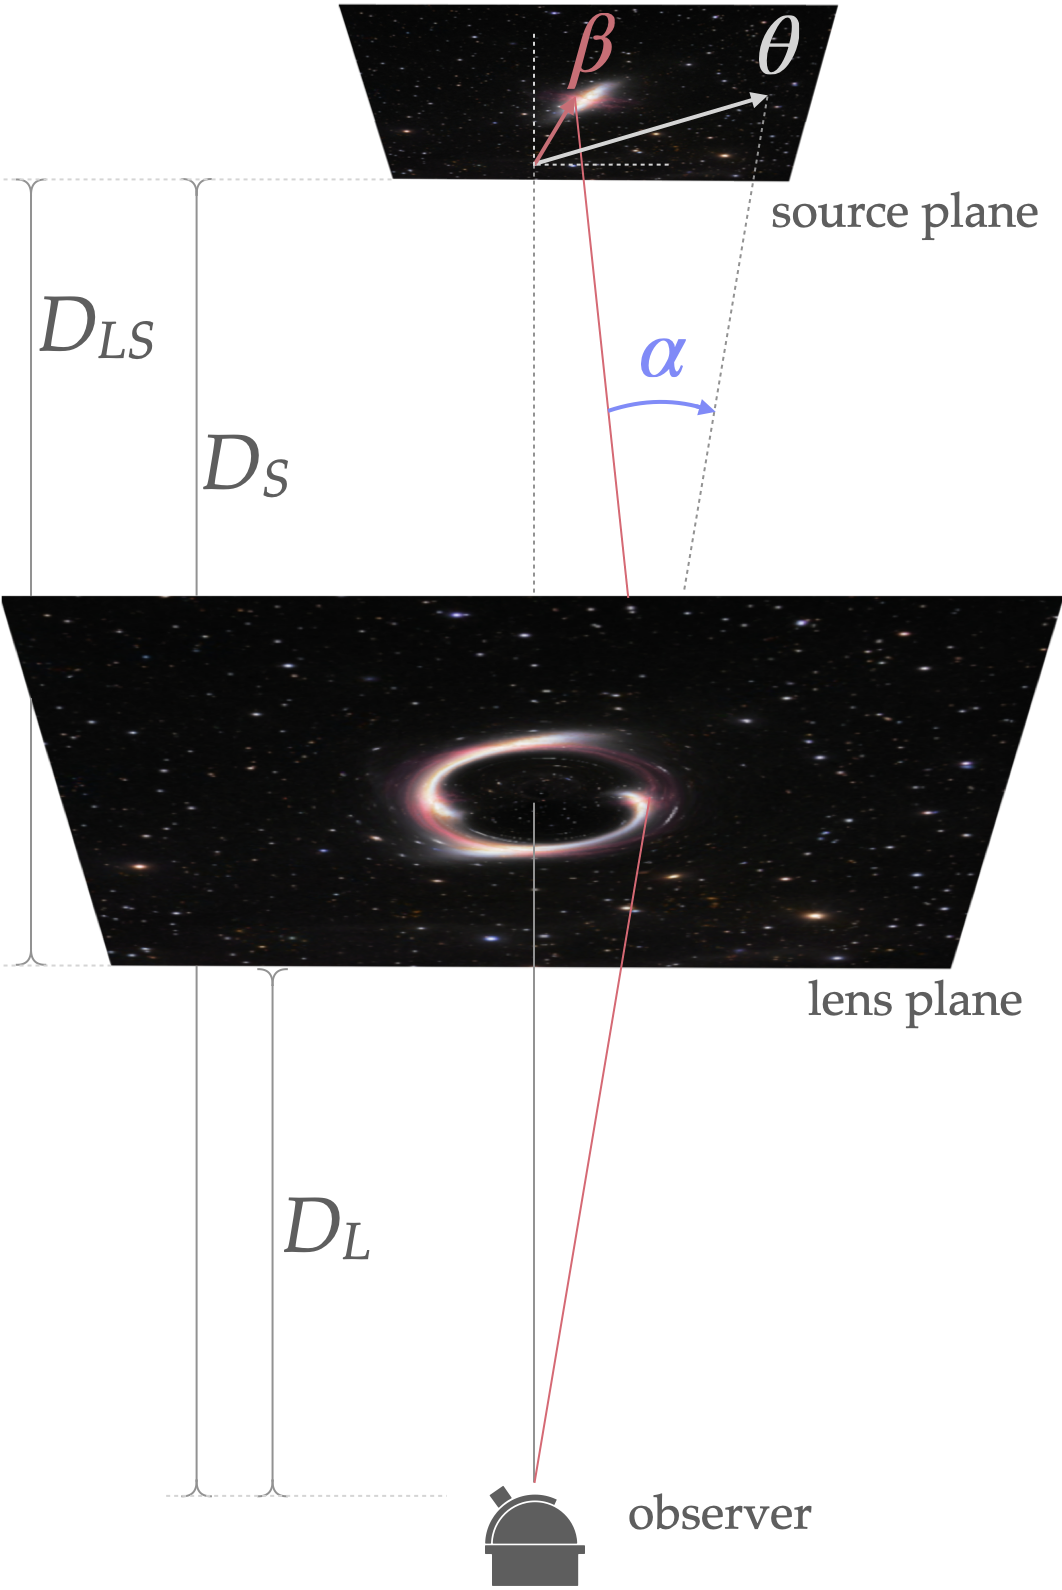
\includegraphics[width=0.8\textwidth]{geometrics}%
  \caption[Lensing geometrics]{A diagram of a lensing system's geometry.  The
  distance to the lens plane is usually measured as an angular diameter distance
  $D_{L}$, and to the source plane as $D_{S}$.  The angular diameter distance
  from the lens plane to the source plane is usually designated with $D_{LS}$.
  From an observer's perspective, images appear to originate from an angular
  position $\bm\theta$ (white), however due to the lens-induced deflection
  $\bm\alpha$ (blue), the true light path (in red) is bent and originates from
  the intrinsic source position $\bm\beta$.  The diagram furthermore suggests
  how the observable position $\bm\theta$ is geometrically composed of the
  unknowns $\bm\beta$ and $\alpha$.}%
  \figlbl{geometrics}%
\end{figure}%

A diagrammatic representation of such a lens configuration and its geometry from
the observer's perspective is shown in \figref{geometrics}.  At any position
$\bm\theta$ (whether an image is observable or not), the travel time of a light
ray from a fixed source position $\bm\beta$, also called arrival time, is given
by the Shapiro time delay on the purely geometrical, unperturbed travel time
\sidecite{Blandford86}
%
\begin{equation}\eqlbl{delay_components}%
  t(\bm\theta) = t_{\text{geom}}(\bm\theta, \bm\beta)
  + \Delta t_{\text{Shapiro}}(\bm\theta).
\end{equation}%
%
As illustrated in \figref{geometrics}, the geometric path is bent by the
deflection angle $\bm\alpha$ and for small values $\alpha\propto(\bm\theta -
\bm\beta)$. Due to the added path length compared to the direct path from the
intrinsic source position, the geometric time delay is proportional to
$\frac{1}{2}(\bm\theta - \bm\beta)^{2}$.  In the observer frame, these time
delays have to be scaled with appropriate factors of angular diameter distances
to the lens $D_{L}$ at a redshift $z_{L}$, to the source $D_\mathrm{S}$ at a
redshift $z_{S}$, and from the lens to the source $D_{LS}$ (see
\figref{geometrics} for details)\sidenote{Note that in a general cosmological
context angular diameter distances are not additive, i.e. $D_{LS} \neq D_{S} -
D_{L}$.}
%
% \begin{equation}\eqlbl{geo_and_shapiro}%
%   \begin{aligned}
%     t_{\text{geom}} &= \frac{(1+z_{L})}{2}\frac{D_{L}D_{S}}{cD_{LS}}(\bm\theta - \bm\beta)^{2} \\
%     \Delta t_{\text{Shapiro}} &= -2\frac{(1+z_{L})}{c}\int_{0}^{z_{S}}\Phi(\bm\theta, z)\,\mathrm{d}z.
%   \end{aligned}
% \end{equation}%
%
\begin{equation}\eqlbl{geo_and_shapiro}%
  \begin{aligned}%
    t_{\text{geom}} &= \frac{(1+z_{L})}{2}\frac{D_{L}D_{S}}{D_{LS}}(\bm\theta - \bm\beta)^{2} \\
    \Delta t_{\text{Shapiro}} &= -2(1+z_{L})\int_{0}^{z_{S}}\Phi(\bm\theta, \zeta)\,\mathrm{d}\zeta,
  \end{aligned}%
\end{equation}%
%
where $\zeta$ is the line-of-sight coordinate.  The distance to the lens and the
source $D_\mathrm{S}$ are always much larger than the line-of-sight extent of
the lens itself. This is what allows the so-called \textit{thin-lens}
approximation which allows the definition of a relativistic two-dimensional (2D)
\textit{lens potential}, the projection of a three-dimensional potential onto
the 'lens plane'
%
% \begin{equation}\eqlbl{lens_potential}%
%   \psi(\bm\theta) = \frac{2D_{LS}}{c^{2}D_{L}D_{S}}\int_{0}^{z_{S}}\Phi(\bm\theta, z)\,\mathrm{d}z.
% \end{equation}%
%
\begin{equation}\eqlbl{lens_potential}%
  \psi(\bm\theta) = \frac{2D_{LS}}{D_{L}D_{S}}\int_{0}^{z_{S}}\Phi(\bm\theta, \zeta)\,\mathrm{d}\zeta,
\end{equation}%
%
Just as the Poisson equation \eqref*{Poisson} in 3D relates the Newtonian
potential to a mass-density distribution, there is a 2D inverse Laplace
operator\sidenote{in integral form the operator is a convolution with the
Green's function $G(\bm\theta') = (2\pi)^{-1}\log{|\bm\theta'|}$} $\nabla^{-2}$
which connects a surface mass-density distribution $\kappa$ to the lensing
potential
%
% \begin{equation}\eqlbl{convergence}%
%   \begin{aligned}
%     \psi(\bm\theta) &= 2\nabla^{-2}\kappa \\
%     \kappa(\bm\theta) &= \frac{4\pi GD_{LS}D_{L}}{c^2D_{S}}
%     \int \rho(\bm\theta, z)\,\mathrm{d}z,
%   \end{aligned}
% \end{equation}%
%
\begin{equation}\eqlbl{convergence}%
  \begin{aligned}
    \psi(\bm\theta) &= 2\nabla^{-2}\kappa \\
    \kappa(\bm\theta) &= \frac{4\pi D_{LS}D_{L}}{D_{S}}
    \int \rho(\bm\theta, \zeta)\,\mathrm{d}\zeta.
  \end{aligned}
\end{equation}%
%
Also called \textit{convergence}, $\kappa$ itself is in fact dimensionless, as
it is in units of the \textit{critical surface density} scaling $\left(4\pi
D_{LS}D_{L}/D_{S}\right)^{-1}$.  It characterises the 'compactness' of a lensing
system and describes a limit beyond which a mass distribution produces multiple
images from a source behind the lens, i.e. a mass and area limit at which a
system is strongly lensing.

% Arrival-time surface
Finally, inserting \eqref{geo_and_shapiro}, \eqref*{lens_potential}, and
\eqref*{convergence} into \eqref{delay_components}, yields the travel times up
to an arbitrary constant as a functional surface of observed angular positions,
called the \textit{arrival-time surface}
%
% \begin{equation}\eqlbl{delay_components}%
%   \begin{aligned}%
%     ct(\bm\theta) &= (1+z_{L})\frac{D_{L}D_{S}}{D_{LS}}\;\tau \\
%     \tau &= \frac{1}{2}(\bm\theta-\bm\beta)^{2} - \psi(\bm\theta).
%   \end{aligned}%
% \end{equation}%
%
\begin{equation}\eqlbl{arrival_time_surface}%
  \begin{aligned}%
    t(\bm\theta) &= (1+z_{L})\frac{D_{L}D_{S}}{D_{LS}}\;\tau \\
    \tau &= \frac{1}{2}(\bm\theta-\bm\beta)^{2} - \psi(\bm\theta),
  \end{aligned}%
\end{equation}%
%
where $\tau$ describes the dimensionless arrival-time surface in cosmological
scaling. While it is a rather abstract construct\sidenote{however, it is closely
related to real-space wavefronts} and is not entirely observable, the study of
$\tau$ and its derivatives cam explain most of a lensing phenomenon.

% Arrival-time surface and derivatives
The first derivative is another formulation of Fermat's principle
%
\begin{equation}\eqlbl{lens_equation}%
  \begin{aligned}%
    \nabla\tau &= 0 \\
    \bm\theta &= \bm\beta + \nabla\psi = \bm\beta + \bm\alpha,
  \end{aligned}%
\end{equation}%
%
where \eqref{deflections} was used to insert $\alpha = \nabla\psi$.  From
\figref{geometrics}, this relation between the deflection, intrinsic source, and
observable source is also evident, and is often called the ray-tracing or
\textit{lensing equation}. \sidenote{The second derivative $\nabla\nabla\tau$ is
the inverse magnification tensor which explains how small displacements in the
source plane take effect on the lens plane.}

% Lensing equation for modelling
The lensing equation is especially important for reconstructing mass
distributions of observations.  The left-hand side of the second equation
\eqref*{lens_equation} is observable and measurable, whereas the right-hand side
terms are unknown and thus have to be modelled.  In general terms, lens
modelling is the process of finding credible mass distributions of lensing
galaxies (or clusters) which are able reproduce the observed deflections of a
background source.  There are several strategies of how one can go about
constructing such mass distributions.  

A very popular approach consists of building parametric models whose shape is
determined by a set of parameters.  The philosophy behind it is to match the
number of parameters to the sparsity of observables.  This often means,
flexibility and complexity is traded for simplicity by eliminating unimportant
parameters, which makes the choice of the right parameters especially crucial.
The advantage of such methods is the high efficiency with which such models can
be generated.  

Contrary to parametric models, free-form models use a much higher number of
parameters usually in form of small components which are superposed to build the
lens.  These components can in principle use of any form basis function such as
Bessel functions or isothermal spheres, however most commonly square mass tiles,
or pixels are used to assemble the lens mass distribution.  The advantage of
free-form methods lies in the flexibility they have to build various shapes of
models, but this is also their most critiqued aspect, as too much flexibility
easily leads to unphysical models which contradict galaxy formation and
evolution theory.  Another rather irrelevant argument usually made against
free-form models is that they tend to hide parameters which describe dominant
features of a lens amongst many less important ones.  

In this context, it is very useful to think of an arbitrary surface-density
distribution in terms of multipoles:
%
\begin{equation}\eqlbl{match:multipoles}%
  \kappa(\bm\theta) = \langle\kappa_0(\theta)\rangle_{\phi} 
  + \sum^{\infty}_{m=1} \langle\kappa_{m}(\theta)\rangle_{\phi} e^{im\phi}
\end{equation}%
%
where the individual components $\langle\kappa_{m}(\theta)\rangle_{\phi}$ are
angular averages over the surface density, expressed in polar coordinates.  It
corresponds much to the idea that galaxies consist of a main body of matter and
many smaller substructures orbiting around it.  The monopole $\kappa_0$, dipole
$\kappa_1$ and quadrupole $\kappa_2$ are usually considered the most important
components.  While the monopole only leads to radial deflections, the
higher-order multipoles also include angular terms which are composed of two
parts containing the interior and exterior poles.  The angular structure in the
lens is mainly determined by three components: (i) the luminous lens galaxy
including its stars, gas, and dust, (ii) the dark matter in the halo of the
galaxy, and (iii) the perturbations from nearby objects or objects along the
line of sight.  The most common angular term included by lens models is the
external shear which describes the exterior poles of the quadrupole.

% Lensing degeneracies
In fact, \sideciteay{Young1980} reported the first lens model which already
involved all components up to the quadrupole expressed in terms of an elliptical
mass distribution using a small set of parameters.  Already then, they
identified essentially every important lensing-related issue, and in particular
realized that there are many different mass distributions which can lead to
identical lensing configurations \sidecite{Young1981a}; these degeneracies
represent an inherent limitation to lens reconstructions \sidecite{Saha2000}.
They create many misconceptions about lens models even amongst experts, as often
times a single family of models is not able to fully describe lensing
observables \sidecite{Gomer19, Kochanek20}.  To reduce or even break
degeneracies, modern lens reconstruction techniques try to constrain their
models with additional data besides the image positions such as relative fluxes
of the images, arc-like extended images, stellar photometry to describe the
dynamics and inner structure of the lensing galaxies, or time delays between the
images \sidecite{Harvey19, Warren03, Barnabe07, Ferreras07, Shajib20}.